\documentclass[11pt,letterpaper]{article}
\usepackage[T1]{fontenc}
\usepackage[utf8]{inputenc}
\usepackage{lmodern}
\usepackage[margin=1in]{geometry}
\usepackage{amsmath,amssymb,amsthm,mathtools}
\usepackage{microtype,booktabs,longtable,tabularx,array}
\usepackage{enumitem,xcolor,graphicx}
\usepackage{listings,xurl,hyperref,bookmark}
\usepackage{fancyhdr}
\definecolor{ink}{HTML}{15324F}
\definecolor{accent}{HTML}{14666B}
\definecolor{muted}{HTML}{5A6570}
\hypersetup{colorlinks=true,linkcolor=ink,citecolor=accent,urlcolor=accent,
 pdftitle={Unknot Recognition by Continuation Quotients and Certified Algebraic Splitting},
 pdfauthor={ProveIt research continuation}}
\pagestyle{fancy}\fancyhf{}
\fancyhead[L]{\small\textcolor{muted}{ProveIt: unknot recognition}}
\fancyhead[R]{\small\textcolor{muted}{Continuation quotients and algebraic splitting}}
\fancyfoot[C]{\thepage}
\setlength{\headheight}{14pt}
\setlength{\emergencystretch}{2em}
\setlist{itemsep=3pt,topsep=5pt}
\lstset{basicstyle=\small\ttfamily,breaklines=true,columns=fullflexible,
 frame=single,rulecolor=\color{muted!35},backgroundcolor=\color{muted!3},
 showstringspaces=false,keepspaces=true}
\newtheorem{theorem}{Theorem}[section]
\newtheorem{lemma}[theorem]{Lemma}
\newtheorem{proposition}[theorem]{Proposition}
\newtheorem{corollary}[theorem]{Corollary}
\newtheorem{definition}[theorem]{Definition}
\newtheorem{example}[theorem]{Example}
\newtheorem{remark}[theorem]{Remark}
\newcommand{\F}{\mathbb F_2}
\newcommand{\N}{\mathbb N}
\newcommand{\Z}{\mathbb Z}
\newcommand{\Q}{\mathbb Q}
\newcommand{\Kh}{\operatorname{Kh}}
\newcommand{\rKh}{\widetilde{\operatorname{Kh}}}
\newcommand{\rank}{\operatorname{rank}}
\newcommand{\End}{\operatorname{End}}
\newcommand{\im}{\operatorname{im}}
\newcommand{\coker}{\operatorname{coker}}
\newcommand{\capthree}{\operatorname{cap}_3}
\newcolumntype{Y}{>{\raggedright\arraybackslash}X}
\newcommand{\code}[1]{\texttt{#1}}
\newcommand{\UNKNOT}{\textup{\textsc{unknot}}}
\newcommand{\KNOTTED}{\textup{\textsc{knotted}}}
\newcommand{\UNKNOWN}{\textup{\textsc{unknown}}}
\newcommand{\pin}{\nolinkurl{eb79136d949a1c0e6f4bd2f07e6b3990d1130632}}
\title{\textcolor{ink}{Unknot Recognition by Continuation Quotients\newline
and Certified Algebraic Splitting}\\[6pt]
\large Short interval models and exact hidden summands\\
A quantitative route to quasi-polynomial time}
\author{Research continuation for the ProveIt project}
\date{8 October 2026}
\begin{document}
\maketitle
\begin{abstract}
We continue the exact ProveIt unknot recognizer with a decision-specific
algebraic quotient and a verified method for splitting hidden summands.
For a direct summand whose differential entries are scalar multiples of one
fixed square-zero endomorphism, classical type-$A$ decomposition produces
interval complexes. We prove that every such interval of length at least
two can be replaced by a two-term interval while preserving the completed
unreduced Khovanov rank capped at three under every remaining tangle
continuation. The proof uses the dual-number identity
\[
 \dim_{\mathbb F_2}H(J_\ell\otimes_A D)
   =a\ell+2\sum_m b_m\min(\ell,m)
\]
over $A=\mathbb F_2[\epsilon]/(\epsilon^2)$, where $J_\ell$ is the free
$\epsilon$-string, and the even-dimensional circle spaces in an ordinary closure. The length
bound is sharp for these observations. Exact homology calculations retain
the original interval lengths.

At a stage where all remaining summands admit this normalization, the number
of physical objects is at most
$P(w)=(w-1)!!\bigl(1+2(2^{2^{w/2}-1}-1)\bigr)$,
independent of interval lengths and virtual multiplicities. If $g$ bounds
the number of crossings between such stages, we obtain
\[
 T(n;w,g)\le n^{O(1)}
  \exp O\!\left(g+w\log(w+1)+2^{w/2}\right).
\]
This is quasi-polynomial under an explicit condition on $w$ and $g$;
no universal bound on these execution parameters is established.

The implementation also solves bounded scalar chain-endomorphism systems
and verifies Fitting decompositions, exposing genuine direct sums inside
connected differential graphs. A separate subset dynamic programme exactly
optimizes crossing windows. Tests include independent dense continuation
calculations, witness replay, complete homology comparisons, and paired
timings. The measurements distinguish fewer algebraic operations from wall
time and distinguish synthetic activation of interval shortening from
observed behavior on actual diagrams. The deliverable includes the article,
source, reference snapshots, integration patches, and reproducible evidence.
\end{abstract}

\clearpage
{\fontsize{9}{10}\selectfont\tableofcontents}
\newpage
\section{Results, scope, and the verified starting point}
\label{sec:scope}

\subsection{The question this continuation answers}
The ProveIt project asks for an exact recognizer whose running time approaches
\begin{equation}\label{eq:target}
 T(n)=n^{O(\log n)}=2^{O((\log n)^2)}
\end{equation}
on an explicitly given classical knot diagram with $n$ crossings. The existing
implementation is complete without resource limits, but its worst-case bound
is exponential. This article develops a specific way of discarding algebraic
information that is irrelevant to the final decision, and a verified way of
exposing direct summands that were hidden by the current choice of basis.

The strongest new statement is an observation theorem. Suppose a genuine
direct summand of the open complex has one crossingless matching $M$ in every
degree and one fixed nonzero nilpotent coefficient $\theta$ in every nonzero
differential entry. First put its scalar coefficient matrices into interval
form. Then, \emph{for the unreduced rank-two unknot decision}, every interval
of length at least two may be replaced by an interval of length two. This
preserves the final total rank capped at three under every remaining crossing
sequence and closure. The replacement is generally not a chain homotopy
equivalence. Its safety follows from a proved property of every allowed
continuation, rather than from agreement on a finite test collection.

The same observation gives an explicit complexity theorem. At a stage whose
residual components all have the stated form, the number of stored objects
after decision compression is bounded solely in terms of the frontier size.
If such stages occur frequently enough, the entire scanner has a
quasi-polynomial bound. The missing universal assertion is now a concrete
structural condition on the intervening residual complexes.

\begin{center}\small
\begin{tabularx}{\textwidth}{@{}>{\raggedright\arraybackslash}p{.25\textwidth}Y>{\raggedright\arraybackslash}p{.23\textwidth}@{}}
\toprule
Contribution & Guarantee & Status\\
\midrule
Interval normalization & Exact chain isomorphism for common-nilpotent direct
summands, with interval counts computed by binary rank invariants & Proved and implemented\\
Length-two decision model & Same completed rank capped at three for every
ordinary Khovanov continuation & Proved and implemented; exact ranks excluded\\
Scalar Fitting splitting & Every accepted split is an exact chain isomorphism,
with complete transformed cross terms checked & Implemented with bounded search\\
Checkpoint complexity & Explicit $2^{O((\log n)^2)}$ sufficient condition in
frontier size and distance between suitable stages & Proved conditional bound\\
Window order optimization & Exact optimum for a chosen window, with a
nonincreasing global combinatorial objective & Proved and implemented\\
General quasi-polynomial recognizer & Bound~\eqref{eq:target} on every input & Not established\\
\bottomrule
\end{tabularx}
\end{center}

\subsection{Repository and artifact provenance}
The inspected ProveIt revision~\cite{proveit} is \pin. Its
\code{Topology/UnknotRecognition/fast} tree has Git identifier
\nolinkurl{b99a666269f660d932fc82ac8d1f29d3ae42231f}.
All forty source, test, example, and configuration files in the preceding
package's unchanged reference directory were independently hashed as Git
blobs and matched to this current tree. Thus the starting implementation is
grounded in repository bytes, rather than a reconstruction from a conversation
summary. The package records both Git blob identifiers and SHA-256 hashes.

The immediate development base is the separately delivered
\emph{Unknot Recognition by Structural Certificates and Compressed Chain
Complexes}, version 0.3.0~\cite{prior}. That package adds signed Seifert-graph
certificates, literal component sharing, multiplicity saturation, and optional
suffix-Euler lower bounds. Those additions are retained in the supplied
version 0.4.0. They are not contributions of the present article.

A concurrent continuation investigated faster factorization, sparse
Alexander calculations, pointed homology, and a three-braid recognizer. The
present package is based on the inspected repository plus the structural
0.3.0 package; it does not claim that the independent branch has been merged
or jointly tested. The two supplied patches distinguish an incremental update
from 0.3.0 and a cumulative update from the pinned repository tree. This makes
the integration boundary explicit.

\subsection{Relation to the two linked research repositories}
We also inspected the \code{openai/math} repository at
\nolinkurl{adc7f1241b42e322a6451854ab7e4b4c146bf78a}. Its catalogue does not
provide a ready-made replacement for the knot recognizer. One nearby theme is
family 116, concerning finite matrix observations of bounded noncommutative
formulas. Its formalization scope distinguishes a division-free hitting
property from separately asserted construction and dimension bounds
\cite{openaimath}. The useful methodological connection is to prove which
finite observations suffice before compressing an algebraic object.

No identity-testing theorem is imported as a Khovanov rank algorithm. A
small formula, a small chain model, and a method for evaluating homology rank
are different inputs. Our continuation theorem explicitly proves the needed
observation property in the dual-number setting, where the relevant derived
category can be classified. That is the substantive bridge to the broader
compressed-algebra theme.

\subsection{Current primary literature and the size of the target}
Lackenby's 2021 lecture material announces
$2^{O((\log n)^3)}=n^{O((\log n)^2)}$ time~\cite{lackenbytalk}. This is
quasi-polynomial, but differs from the stronger target~\eqref{eq:target} used
in this project. His July 2026 preprint gives a new hierarchy algorithm and
efficient certification results. Section 9 expressly treats an iteration
bound separately from an implementation time bound; Proposition 9.1 gives
$L(g+1)^L$ iterations in its hierarchy parameters~\cite{lackenby2026}.
The sources inspected do not supply an end-to-end quasi-polynomial
implementation of the geometric route. This article advances the existing
algebraic scanner.

A particularly relevant obstruction is the 2026 work of Kelom\"aki and
Sch\"utz. Their Theorem 1.2 proves exponential behavior of the explicit
Bar-Natan scanning and divide-and-conquer algorithms even on positive or
alternating three-braids. Their separate special-purpose result computes
three-braid homology in polynomial time~\cite{kelomaki}. Thus a bound on
boundary matching types alone cannot control the number of basis objects or
the differential data between them. Both multiplicity compression and
compression within a single connected component matter.

The classical inputs here are the tangle construction and local cobordism
relations~\cite{khovanov,barnatan}, type-$A$ interval decomposition
\cite{carlsson}, and the derived classification over the dual numbers
\cite{keller}. We give proofs of the algebraic statements actually used.
We make no literature-wide priority claim for barcode decomposition, Fitting
decomposition, or the classification itself. The contribution is their
specific continuation quotient, verified implementation, and quantified
application to this recognizer.

\subsection{Encoding and validation conventions}
The input is an explicitly listed planar-diagram code, or a braid/grid
description converted to such a code. Public command-line input is validated
as a one-component classical spherical diagram. The low-level scanner APIs
retain the inherited validity promise. An empty diagram denotes one
crossing-free circle, with unreduced rank two. Normalized edge labels require
$O(n\log(n+2))$ input bits. Arbitrarily long supplied labels also incur their
reading and normalization cost.

All new algebra is over $\F$. The scanner forgets quantum degree and retains
raw cube homological degree in exact-rank mode. In decision mode, uniform
homological shifts and then interval lengths may be discarded only for the
proved total-rank observation. The distinction is reflected in separate
return schemas: \code{rank} and \code{by\_degree} are exact, whereas
\code{rank\_capped} records only a threshold result. A resource limit produces
\UNKNOWN, never a mathematical verdict inferred from an unfinished scan.

\section{The algebraic model and the decision threshold}
\label{sec:algebraic-model}

The input is an explicitly listed, validated classical knot diagram with
$n$ crossings. Complexity statements use normalized edge labels of
$O(\log(n+2))$ bits; reading and normalizing a longer external encoding
incurs its actual input-size cost. The empty input denotes one
crossing-free circle. A scan
order determines, after each crossing, a finite set of live boundary
labels. Its cardinality is even. As in the preceding implementation, the
objects of the scanning category are loopless matchings of these labels;
closed circles are replaced by their two summands by delooping. We retain
homological degrees and work over $\F$, but forget the quantum grading.
In particular, the basis changes below are assertions in the
quantum-ungraded category. A quantum-graded extension would require
additional compatibility conditions on those basis changes.

Write
\[
 r_2(K)=\dim_{\F}\Kh(K;\F).
\]
The decision criterion used by the existing recognizer is
\begin{equation}\label{eq:rank-two}
 K\text{ is an unknot}\quad\Longleftrightarrow\quad r_2(K)=2.
\end{equation}
Here is the coefficient justification. The reduced/unreduced splitting
over $\F$ gives $r_2(K)=2\dim_{\F}\rKh(K;\F)$
\cite{shumakovitch}. The universal coefficient theorem implies
\[
 \dim_{\Q}\rKh(K;\Q)\le\dim_{\F}\rKh(K;\F).
\]
The rational-rank unknot-detection theorem then excludes every nontrivial
knot when the reduced $\F$ rank is one~\cite{km}. The reverse implication
follows from the unknot complex. This argument does not assume that a
rank-one reduction modulo two excludes odd integral torsion.

We use the notation
\[
 \capthree(a)=\min(3,a),\qquad a\in\N.
\]
A completed capped value of two therefore certifies \UNKNOT, while a
value of three certifies \KNOTTED. For a valid knot the latter value means
that the actual rank is at least four. Values zero and one indicate a
violated input promise or an implementation invariant; they are not
interpreted as topological verdicts.

The algebraic correctness statements are relative to the established
Bar--Natan gluing, delooping, and cancellation operations
\cite{khovanov,barnatan}. The new algorithms operate on their finite
matrices and use exact binary arithmetic. They do not constitute a formal
verification of the entire topological foundation.

\section{Exact interval normalization of square-zero components}
\label{sec:interval-normalization}

\subsection{A recognizable coefficient subcategory}

For a matching $m$ with $k$ arcs, the endomorphism ring used by the scanner
is the dot algebra
\begin{equation}\label{eq:dot-algebra}
 R_m=\End(m)\cong
 \F[x_1,\ldots,x_k]/(x_1^2,\ldots,x_k^2).
\end{equation}
Its binary basis consists of the squarefree dot monomials; its dimension
is $2^k$. The identity is the constant monomial. This is the familiar
diagonal endomorphism algebra of the matching category
\cite{khovanov,barnatan}.

Let $\mathfrak m=(x_1,\ldots,x_k)$ be the augmentation ideal. Every
$\theta\in\mathfrak m$ satisfies $\theta^2=0$: in characteristic two,
the square of a sum is the sum of its squares, and each nonconstant
squarefree monomial has square zero. Conversely, an element with constant
coefficient one is a unit. Thus the nonzero augmentation elements are
exactly the nonzero nonunits of this ring.

The undirected differential graph has one vertex per object and an edge
when a differential entry is nonzero. Its connected components are
literal direct summands of the complex. The earlier sharing backend
identifies repeated components by complete serialization~\cite{prior}.
The following condition exposes additional summands inside such a
component.

\begin{definition}[Pure component]\label{def:pure}
A nonsingleton differential component is \emph{pure} if all its objects
have one matching $m$ and every nonzero differential entry is one fixed
nonzero $\theta\in R_m$ satisfying $\theta^2=0$. A singleton is pure
without a choice of $\theta$.
\end{definition}

Purity is a test of the actual stored matrix. We do not posit an oracle
which determines whether an arbitrary complex can be made pure. In a pure
component, write the degree-$h$ term as $m^{d_h}$. Then
\begin{equation}\label{eq:theta-matrix}
 \delta_h=\theta M_h,\qquad
 M_h:\F^{d_h}\longrightarrow\F^{d_{h+1}},
\end{equation}
where $\delta_h$ is the differential and $M_h$ is a binary matrix.
The matrices $M_h$ need not satisfy
$M_{h+1}M_h=0$. The actual differential squares to zero because
$\theta^2=0$. The distinction is essential for the algorithm: its rank
calculations use products of the $M_h$, not products of the actual
cobordism differentials.

\begin{definition}[Interval complex]
For integers $a\le b$, let $I_{[a,b]}(m,\theta)$ have one copy of $m$ in
each degree $a,\ldots,b$, with differential $\theta$ between successive
copies and zero elsewhere. Its length is $b-a+1$. After removing the birth
shift $a$, write this complex as $I_{b-a+1}(m,\theta)$.
\end{definition}

\subsection{The exact decomposition and its computation}

\begin{theorem}[Exact interval normalization]\label{thm:interval}
Every pure component is chain-isomorphic to a direct sum of interval
complexes. The isomorphism is given by binary changes of basis within
each homological degree. The interval multiplicities are uniquely
determined by the binary matrices in~\eqref{eq:theta-matrix}.
\end{theorem}

\begin{proof}
We first prove the elementary interval decomposition for an arbitrary
finite sequence of binary vector spaces and maps $M_h$; this is the
equioriented type-$A$ case of the usual interval classification
\cite{carlsson}. Suppose the sequence is nonzero. Let $a$ be its earliest
nonzero degree, and choose the largest $b\ge a$ for which the composite
from $V_a$ to $V_b$ is nonzero, counting the identity when $b=a$.
Choose $v_a$ whose image $v_b$ is nonzero, and let $v_h$ be its successive
images for $a\le h\le b$. Choose a covector $\lambda_b$ with
$\lambda_b(v_b)=1$, and define
\[
 \lambda_h=\lambda_bM_{b-1}\cdots M_h,
 \qquad p_h=v_h\lambda_h\quad(a\le h\le b).
\]
Outside this interval put $p_h=0$. We have $\lambda_h(v_h)=1$, so each
$p_h$ is idempotent. For an interior arrow,
$p_{h+1}M_h=M_hp_h$. At the left endpoint $V_{a-1}=0$; at the right
endpoint $M_bv_b=0$ by maximality of $b$. Hence $p$ is an idempotent
endomorphism of the entire sequence. Its image is one interval and its
kernel is an invariant complement. Induction on the total vector-space
dimension proves existence.

Every binary invertible change-of-basis matrix remains invertible after
its entries are multiplied by $\mathrm{id}_m$ in the additive category:
its binary inverse supplies the actual inverse. Applying the changes
of basis to $\theta M_h$ therefore gives a chain isomorphism of the
original component with the corresponding $\theta$-intervals.
The multiplicity formula below proves uniqueness.
\end{proof}

Let the occupied degree range be $u,\ldots,v$. For $u\le a\le b\le v$
define the rank invariant
\begin{equation}\label{eq:rank-invariant}
 \rho(a,b)=\rank(M_{b-1}\cdots M_a),
 \qquad \rho(a,a)=d_a.
\end{equation}
Ranks with an endpoint outside the occupied range are assigned the value
zero. An interval $[p,q]$ contributes one to $\rho(a,b)$ exactly when
$p\le a\le b\le q$. Taking successive differences gives
\begin{equation}\label{eq:mobius-bars}
 \mu(a,b)=\rho(a,b)-\rho(a-1,b)
          -\rho(a,b+1)+\rho(a-1,b+1).
\end{equation}
This is the multiplicity of $[a,b]$. In particular, the result is a
nonnegative integer, and
\begin{equation}\label{eq:barcode-audit}
 \sum_{a\le b}\mu(a,b)(b-a+1)=\sum_h d_h.
\end{equation}
These identities give both a deterministic algorithm and useful
independent consistency checks. The implementation can compute all ranks
by binary matrix multiplication and elimination, form the differences,
and reconstruct the rank invariant from the resulting intervals.

If there are $H$ degree layers and $B$ objects, a conservative elementary
bound is $O(H^2B^3)$ binary field operations. No efficiency claim depends
on this exponent being optimal. Bit-packed matrices provide the practical
implementation. Recognition of purity and the required coefficient
comparisons are polynomial in the stored matrix and coefficient lengths.

Replacing the component by explicit intervals retains exactly $B$ objects
by~\eqref{eq:barcode-audit}. Its advantage is that these objects now lie
in separately shareable summands. Number an interval's vertices in
increasing degree, and remove its birth shift. Its complete template is
then determined by $(m,\theta,\text{length})$. Length-one templates do not
use $\theta$. Equal templates can be continued once, with exact shifted
multiplicities or with the existing saturated multiplicities.

\begin{example}[A strict improvement over graph-component sharing]
\label{ex:dense-pure}
Take $B\ge2$ copies of $m$ in degree zero and $B$ copies in degree one,
and put $\theta$ in every differential entry. Its differential graph is
the connected graph $K_{B,B}$, and no entry is a unit. Literal component
sharing leaves one template with $2B$ objects. The scalar matrix is the
all-ones matrix of rank one. Interval normalization produces one
length-two interval and $B-1$ singletons in each of the two degrees.
After shifted sharing, only three objects remain: two in the interval
and one singleton with multiplicity polynomial $(B-1)(1+z)$.

This is a valid algebraic stress family. It is not asserted that arbitrary
members occur as intermediate states of the current knot scanner. That
additional realizability assertion would need a separate construction.
\end{example}

The replacement must apply to an entire direct summand. A tower attached
to other matchings may be normalized only if its basis changes are also
applied to every external incident differential. Simply discarding those
attachments would invalidate the complex. The exact splitter developed
in the next part of the article addresses this issue by producing and
checking an actual change of basis.

\section{Short intervals with identical capped continuation ranks}
\label{sec:continuation-quotient}

Exact normalization still leaves intervals of unbounded length. They
need not split further: finite free strings are indecomposable over the
dual numbers~\cite{keller}. The decision problem permits a different operation. A long
string can be replaced by a short one when every possible remaining
continuation has the same capped homology rank. Such a replacement is
not asserted to be a chain-homotopy equivalence.

\subsection{The dual-number tensor calculation}

Put $A=\F[\epsilon]/(\epsilon^2)$, and let $J_l$ be the complex of $l$
copies of the free rank-one $A$-module, in consecutive degrees, with every
differential multiplication by $\epsilon$. All tensor products of
complexes below are totalized, and all dimensions refer to total
$\F$-homology. Homological shifts do not affect these dimensions.

\begin{lemma}[Tensor pairing of intervals]\label{lem:interval-tensor}
For positive integers $l,m$,
\[
 \dim_{\F}H(J_l\otimes_A J_m)=2\min(l,m),
 \qquad
 \dim_{\F}H(J_l\otimes_A\F)=l.
\]
\end{lemma}

\begin{proof}
For the first formula, identify the $lm$ free basis positions of the
total tensor product, after forgetting their grading, with
\[
 R=\F[u,v]/(u^l,v^m).
\]
The total differential on $A\otimes_{\F}R$ is multiplication by
$\epsilon$ times the linear operator $T$ given by multiplication by
$u+v$ on $R$. There are no sign distinctions in characteristic two.
This differential has binary rank $\rank(T)$, so its total homology has
dimension $2lm-2\rank(T)=2\dim\coker(T)$. But
\[
 \coker(T)\cong
 \F[u,v]/(u^l,v^m,u+v)
 \cong\F[u]/(u^{\min(l,m)}),
\]
which has dimension $\min(l,m)$. Collecting the degreewise matrices
into one graded total differential preserves the sum of their ranks.
For the second formula, $\epsilon$ acts by zero on the simple module,
so all differentials vanish and there are $l$ one-dimensional terms.
\end{proof}

The needed derived-category classification is particularly small. Every
bounded complex of finite $A$-modules is isomorphic in the bounded
derived category to a finite direct sum of shifts of the $J_m$ and shifts
of the simple module $\F$~\cite[Example 3.7(b)]{keller}.
Appendix~\ref{app:dual-number-classification} gives an elementary proof
using minimal free resolutions and the finite interval argument above.
We use this established classification as an algebraic input; no novelty
claim is made for it.

\begin{theorem}[The continuation rank formula]\label{thm:rank-formula}
Let $D$ be a bounded complex of finite-dimensional $A$-modules. There are
nonnegative integers $a,b_1,b_2,\ldots$, only finitely many nonzero, such
that, for every $l\ge1$,
\begin{equation}\label{eq:continuation-rank-formula}
 r_l(D):=\dim_{\F}H(J_l\otimes_A D)
   =a l+2\sum_{m\ge1}b_m\min(l,m).
\end{equation}
The integer $a$ counts the simple-module summands of $D$, and $b_m$
counts its free interval summands of length $m$, ignoring shifts.
\end{theorem}

\begin{proof}
The complex $J_l$ is bounded and free, hence tensoring with it preserves
quasi-isomorphisms and computes the derived tensor product. Decompose
$D$ as above and apply Lemma~\ref{lem:interval-tensor} to each summand.
The decomposition is finite, and homology dimensions add under direct
sums. This proves the formula simultaneously for all $l$.
\end{proof}

The theorem does not require the algorithm to compute the decomposition
of the potentially enormous suffix $D$. It proves an identity for every
such suffix, which justifies a local replacement before the suffix is
processed.

\begin{corollary}[Universal length cutoff]\label{cor:universal-cutoff}
For any positive integer threshold $c$, any $D$ as above, and any $l\ge1$,
\[
 \min(c,r_l(D))=\min(c,r_{\min(l,c)}(D)).
\]
In particular, length three is a safe cutoff for rank capped at three
under arbitrary bounded dual-number continuations.
\end{corollary}

\begin{proof}
Only $l\ge c$ needs consideration. If $a>0$, both ranks are at least
$c$. If $a=0$ and some $b_m>0$ has $m\ge c$, that summand contributes
at least $2c$ to both ranks. Otherwise every nonzero $b_m$ has $m<c$,
so the right side of~\eqref{eq:continuation-rank-formula} has stabilized
by $l=c$ and the two ranks are exactly equal.
\end{proof}

The cutoff in this fully general statement cannot be lowered uniformly:
for $D=\F$, the rank is $r_l(D)=l$. The geometric continuations of the
scanner have an extra parity property, which permits a sharper cutoff.

\subsection{Why a tangle continuation has the required module structure}

Fix a matching $m$ and a square-zero endomorphism $\theta$. Let $F$ mean
attach all remaining crossing complexes, close the diagram, and apply
the ordinary unreduced Frobenius TQFT. For the proof, use the strict raw
complex before optional Gaussian contractions. Planar gluing of complexes
is additive, preserves composition, and uses the total tensor
differential~\cite{barnatan}. Thus
\[
 D=F(m),\qquad \epsilon\cdot v=F(\theta)(v)
\]
defines a bounded complex of finite $A$-modules: $F(\theta)$ is a
degree-zero chain map and $F(\theta)^2=F(\theta^2)=0$. Inspecting the
totalized differential gives
\begin{equation}\label{eq:functor-tensor}
 F\bigl(I_l(m,\theta)\bigr)\cong J_l\otimes_A D.
\end{equation}
This identifies the balanced module action required by
Theorem~\ref{thm:rank-formula}. It is stronger than merely saying that
the continuation is a linear operation. The implementation may perform
homotopy-preserving contractions, but the raw functor supplies this
strict model for the proof.

\begin{lemma}[Even continuation rank]\label{lem:even-suffix}
If $m$ admits a nonzero square-zero endomorphism, then
$\dim_{\F}H(F(m))$ is even for every actual scanner continuation.
\end{lemma}

\begin{proof}
The empty matching has endomorphism ring $\F$, so $m$ has at least one
arc. Every complete smoothing of the suffix, glued to $m$, is a nonempty
union of circles. Its unreduced TQFT vector space has dimension $2^c$
for some $c\ge1$. Hence the raw total chain dimension of $F(m)$ is even.
For any finite complex of binary vector spaces,
\[
 \dim H(D)=\dim D-2\rank(d_D),
\]
so its total homology dimension has the same parity. This proves the
claim. In particular, the argument does not require a marked-point
implementation or an assumption that the $A$-module complex is free.
\end{proof}

\begin{theorem}[Geometric length cutoff two]\label{thm:geometric-cutoff}
For every matching $m$, nonzero square-zero $\theta\in\End(m)$, positive
length $l$, and actual remaining continuation $F$,
\begin{equation}\label{eq:length-two}
 \capthree\!\left(\dim H(F(I_l(m,\theta)))\right)
 =
 \capthree\!\left(\dim H(F(I_{\min(l,2)}(m,\theta)))\right).
\end{equation}
\end{theorem}

\begin{proof}
By Lemma~\ref{lem:even-suffix} and
\eqref{eq:continuation-rank-formula},
$r_1(D)=a+2\sum_m b_m$ is even, so $a$ is even. Suppose $l\ge2$.
If $a>0$, then $a\ge2$ and its contribution at length two is already
at least four. If $a=0$ but some $b_m>0$ has $m\ge2$, that summand
also contributes at least four at length two. In the remaining case,
only $b_1$ can be nonzero, and $r_l(D)=2b_1$ is independent of $l$.
These three cases prove the equality. Length one is unchanged.
\end{proof}

\begin{example}[The geometric cutoff is sharp]\label{ex:cutoff-sharp}
Let $m$ pair four cyclically ordered endpoints as
$(1,2)$ and $(3,4)$, and close it with the other crossingless pairing
$(1,4)$ and $(2,3)$. The closure is one circle. Write $x_1,x_2$ for dots
on the two arcs of $m$ and set $\theta=x_1+x_2$. Under closure both dots
act by the same circle operator $x$, so $F(\theta)=x+x=0$. The image
of $m$ is the two-dimensional circle space. Consequently
\[
 \dim H(F(I_l(m,\theta)))=2l.
\]
Replacing a length-two interval by a singleton would change a capped
value of three to two. Thus cutoff one cannot preserve these geometric
observations uniformly. This example concerns valid algebraic objects
and a crossingless planar closure; it does not claim that each source
interval is itself the full complex of a knot diagram.
\end{example}

\subsection{Compositional correctness of the decision backend}

\begin{definition}[Continuation equivalence]\label{def:continuation-equivalence}
For two complexes $C,C'$ on the same boundary, write $C\equiv_3 C'$ if
every permitted remaining crossing sequence and ordinary closure $F$
satisfies
\[
 \capthree\!\left(\dim H(F(C))\right)
 =\capthree\!\left(\dim H(F(C'))\right).
\]
\end{definition}

This is an equivalence relation by equality of the specified observations.
It is preserved by adjoining a common direct summand, taking finitely
many copies, and performing a common crossing extension: in the last
case, any further completion is also a permitted completion before that
extension. Theorem~\ref{thm:geometric-cutoff} identifies long intervals
with length-two representatives for this relation. It does not identify
their homotopy types.

The prior backend stores a template together with nonnegative
multiplicities, optionally recording absolute shifts in a polynomial
$p(z)\in\N[z]$~\cite{prior}. For total-rank decisions, replace the
weight by $\capthree(p(1))$. Addition and multiplication use saturation:
\[
 a\oplus b=\min(3,a+b),\qquad a\otimes b=\min(3,ab).
\]
The map $\N\to\{0,1,2,3\}$ given by saturation preserves both
operations. These are nonnegative counts, not coefficients reduced
modulo two.

\begin{theorem}[Decision correctness under repeated replacements]
\label{thm:decision-correctness}
Start with the existing exact scanning complex. At any stages, perform
exact unit cancellations, exact changes of basis, direct-summand
decompositions, and sharing of equal normalized templates. For each
pure summand, apply Theorem~\ref{thm:interval}; in decision mode shorten
each resulting interval to length $\min(l,2)$ and saturate its
multiplicity at three. Assume that structural choices do not depend on
the discarded multiplicities or absolute shifts. At final closure the
reported count is precisely $\capthree(r_2(K))$.
\end{theorem}

\begin{proof}
Fix the full future crossing order at any proposed replacement. By
Theorem~\ref{thm:geometric-cutoff}, completing a single replaced interval
would give the same capped total homology rank. Completion is additive
on independent summands and commutes with homological shifts. Since
capping commutes with addition and multiplication of nonnegative
integers, replacing any number of independent copies preserves the
capped rank of the completed whole complex. Exact changes of basis,
contractions, and component sharing preserve the actual homotopy type
before capping and hence preserve this observation as well.

Repeat this argument at every later replacement, comparing the
counterfactual full completion immediately before and immediately after
it. Transitivity shows that all replacements together preserve the
capped final rank. At closure, the empty matching has endomorphism
ring $\F$; complete elimination leaves isolated generators, whose
capped multiplicities compute that rank. Finally apply
\eqref{eq:rank-two} for the verdict.
\end{proof}

This proof deliberately uses an observational invariant after shortening.
The represented complex need not retain the original homotopy type,
exact rank, or degree-by-degree homology. The exact-rank backend therefore
uses interval splitting without shortening. The decision backend reports
a capped rank and does not supply exact homological counts or cycle
representatives. Likewise, exact signed Euler data from the former
representation cannot silently be carried through an interval shortening.

The current length alone does not give a completed rank bound greater
than two. For a geometric example, take one arc $m$ with $\theta=x$ and
close it to one circle. Then $D=A$ with $\epsilon$ acting by $x$, and
Lemma~\ref{lem:interval-tensor} gives
$\dim H(J_l\otimes_A A)=2$ for every $l$. Thus arbitrarily long legal
interval complexes can have a rank-two closure observation. For
arbitrary module continuations, an acyclic $D$ can even give rank zero.
The theorem says that the short representative has the same completed
threshold observation; it does not license a verdict from the current
number of stored objects.

\section{A checkpoint bound independent of component size}
\label{sec:checkpoint-complexity}

\subsection{The state count after normalization}

Fix the implemented ordering and exact splitting policy. Let $w$ be the
largest frontier size over the entire planned scan. Let a \emph{pure
checkpoint} be a stage at which, after unit elimination and the chosen
exact splitting operations, every differential component satisfies
Definition~\ref{def:pure}. Include the initial and final states among
the checkpoints. Let $g$ bound the number of crossings between
successive checkpoints. A checkpoint is recognizable from its current
matrix. A useful uniform bound on their gaps is an additional theorem
about an input family, not something implied by their definition.

For even $w\ge0$ put
\begin{equation}\label{eq:M-N}
 M(0)=1,\qquad M(w)=(w-1)!!\quad(w>0),
 \qquad N(w)=2^{\,2^{w/2}-1}-1.
\end{equation}
There are at most $M(w)$ frontier matchings. The quantity $N(w)$ counts
the nonzero augmentation elements of the endomorphism ring of a
matching with $w/2$ arcs: its $2^{w/2}-1$ nonconstant basis monomials
have arbitrary binary coefficients. In particular, $N(0)=0$.
Counting all perfect matchings avoids assuming that the frontier bounds
one disc or that numeric labels specify a useful cyclic order.

\begin{samepage}
\begin{proposition}[Physical size at a pure checkpoint]
\label{prop:checkpoint-size}
After interval normalization, length cutoff two, and complete sharing,
a pure checkpoint satisfies
\begin{equation}\label{eq:checkpoint-P}
\begin{aligned}
 \text{stored templates}&\le M(w)(1+N(w)),\\
 \text{stored objects}&\le P(w):=M(w)(1+2N(w)),
\end{aligned}
\end{equation}
independently of multiplicities and of the sizes of the
original connected differential components.
\end{proposition}
\end{samepage}

\begin{proof}
For each matching there is one possible singleton type, with one object.
Every other retained interval has length two and is determined by its
matching and one of the at most $N(w)$ possible nonzero square-zero
endomorphisms. It contributes two objects. Constructing the vertices
in degree order makes equal triples have equal complete serializations;
no graph-isomorphism oracle is needed for these types. Summing these
counts gives the bounds. A smaller actual frontier only decreases
both $M$ and $N$.
\end{proof}

For comparison, the exact-rank version retains lengths up to $n+1$,
because every raw cube degree lies between zero and $n$. Its analogous
object bound is
\begin{equation}\label{eq:exact-checkpoint-P}
 P_{\mathrm{exact}}(n,w)
 \le M(w)\left(1+N(w)\frac{n(n+3)}2\right),
\end{equation}
using $\sum_{l=2}^{n+1}l=n(n+3)/2$. Absolute birth shifts are recorded
in the exact multiplicity polynomials. The universal cutoff-three
variant for arbitrary module continuations, if desired, has the
decision bound $M(w)(1+5N(w))$ instead of~\eqref{eq:checkpoint-P}.

\subsection{Complexity through impure stretches}

\begin{theorem}[Quantified checkpoint complexity]
\label{thm:checkpoint-complexity}
Under the preceding assumptions, both the exact interval-sharing
backend and the shortened decision backend admit the conservative
bit-complexity bound
\begin{equation}\label{eq:checkpoint-runtime}
 T(n;w,g)\le n^{O(1)}
 \exp\!\left(O\!\left(g+w\log(w+1)+2^{w/2}\right)\right).
\end{equation}
The same expression is a conservative space bound. Exact splitting
operations that preserve the number of objects and cost polynomial
time in the physical matrix size and coefficient dimension may be
included without changing this form of bound.
\end{theorem}

\begin{proof}
In one crossing extension, each old loopless matching has two
smoothings. Each smoothing creates at most two new circles, since every
new circle contains one of the two newly added smoothing arcs. Delooping
therefore creates at most four objects per smoothing, or eight objects
per old object in total. Elimination removes objects; exact basis
changes and interval normalization do not increase their total number;
sharing and shortening only decrease it. Thus, between two checkpoints,
the physical object count is bounded by $8^g$ times the preceding
checkpoint bound, allowing an immaterial additional factor eight
depending on endpoint accounting.

Unit elimination uses polynomially many matrix and coefficient
operations in this physical size. The interval algorithm has
polynomial cost by~\eqref{eq:rank-invariant}--\eqref{eq:mobius-bars}.
The same is true of the exact splitting procedures admitted in the
statement. In the dot-mask algebra, morphisms have $2^{O(w)}$ coefficient
bits, and direct enumeration of monomials and their gluings gives a
conservative $2^{O(w)}$ bit cost per composition or transfer, including
the four temporary ports of the next crossing. This is the same finite
algebra cost model used in the prior analysis~\cite{prior}.

Exact multiplicity polynomials have at most $n+1$ degree positions.
The virtual unreduced allocation grows by at most eight per crossing,
so each coefficient has $O(n)$ bits. In decision mode the weights have
constant size. Complete key comparisons, matching identifiers, and
persistent caches add polynomial factors in the stated physical size
and $n$; the bound need not rely on average-case hashing.

Finally,
\[
 \log M(w)=O(w\log(w+1)),\qquad
 \log(1+N(w))=O(2^{w/2}).
\]
Substitute either~\eqref{eq:checkpoint-P} or
\eqref{eq:exact-checkpoint-P} into the physical-size estimate, charge
the polynomial operations across $n$ crossings, and absorb the
resulting fixed powers in the exponential. This gives
\eqref{eq:checkpoint-runtime}.
\end{proof}

\begin{corollary}[A specific quasi-polynomial regime]
\label{cor:checkpoint-quasipolynomial}
Suppose a diagram family has constructible scan orders and a proved
checkpoint schedule for which
\begin{equation}\label{eq:checkpoint-qp-condition}
 g+2^{w/2}+w\log(w+1)=O(\log^2(n+2)).
\end{equation}
If constructing the order and schedule costs at most $n^{O(\log n)}$
bit operations, the resulting complete recognizer runs in
$n^{O(\log n)}$ bit operations on that family. Fixed $w$ and fixed $g$
give a polynomial bound when the order is polynomial-time constructible.
\end{corollary}

For integer $w$, the last term in~\eqref{eq:checkpoint-qp-condition}
can be absorbed into a universal multiple of $2^{w/2}$; it is displayed
to retain the actual matching-count contribution. For example,
$w\le4\log_2\log(n+2)+O(1)$ and $g=O(\log^2(n+2))$ suffice.

The previous component-sharing theorem required a bound on the maximum
post-elimination connected component size $b$, with the sufficient
condition $b^2 2^{w/2}=O(\log^2 n)$~\cite{prior}. The new result removes
that component-size requirement at pure checkpoints. In particular,
an interval can have length proportional to $n$, and a connected pure
component can contain arbitrarily many copies mixed by binary changes
of basis. Neither prevents the checkpoint bound. The exact and decision
variants achieve this in different ways: exact normalization keeps
polynomially many possible lengths, while the continuation quotient
uses only two lengths.

This remains a conditional structural theorem. No argument here shows
that every knot diagram, or every prime nonhomogeneous diagram left
after the structural front end, has frequent pure checkpoints. Taking
only the initial and final checkpoints can leave $g=n$, which yields
an exponential bound. Likewise, a large frontier remains costly because
$N(w)$ is doubly exponential in $w$. Experimental success of an exact
splitter on individual diagrams is useful evidence about these
parameters, but does not replace the missing uniform theorem.

\subsection{A sharper bound for restricted coefficient alphabets}
\label{sec:coefficient-alphabets}

The all-polynomials count $N(w)$ is deliberately conservative. It can be
replaced when the coefficients occurring at the useful checkpoints have
additional structure. The restriction need only hold at those
checkpoints; arbitrary intermediate coefficients are still charged at
their full dot-mask size.

\begin{corollary}[Checkpoint coefficient alphabets]
\label{cor:coefficient-alphabet}
Suppose that, at every pure checkpoint and for each actual matching $m$,
all nonsingleton pure components use coefficients from a set
$\Theta_{i,m}$ with
\[
 |\Theta_{i,m}|\le A(w).
\]
The sets may depend on the checkpoint $i$ and matching $m$; only their
cardinality bound must be uniform. Under the other assumptions of
Theorem~\ref{thm:checkpoint-complexity}, the decision checkpoint has at
most $M(w)(1+2A(w))$ objects, and both the exact and decision variants
admit the bound
\begin{equation}\label{eq:alphabet-runtime}
 T(n;w,g,A)\le n^{O(1)}
 \exp\!\left(O\!\left(g+w\log(w+1)+\log(1+A(w))\right)\right).
\end{equation}
\end{corollary}

\begin{proof}
For each matching, retain one singleton type and at most $A(w)$
length-two types, giving the stated object count. The exact variant
again gains only a polynomial factor in $n$ from possible lengths.
Between checkpoints the same factor $8^g$ bounds expansion. Importantly,
we still charge $2^{O(w)}$ bit operations for general coefficient
compositions and transfers; we do not assume that low-complexity
coefficients remain so between checkpoints. Its logarithmic contribution
$O(w)$ is absorbed by $O(w\log(w+1))$ for positive even $w$, and the
empty-frontier case is constant. Substitution in the preceding proof
gives~\eqref{eq:alphabet-runtime}.
\end{proof}

For example, put $p=w/2$. If every checkpoint coefficient is a nonzero
\emph{linear} combination of the $p$ dot generators, then
\[
 A(w)\le2^p-1,
 \qquad
 T\le n^{O(1)}\exp O\!\left(g+w\log(w+1)\right).
\]
More generally, if every such coefficient has dot degree at most a
fixed positive integer $d$, the squarefree monomial basis gives
\begin{equation}\label{eq:degree-alphabet}
 A(w)\le2^{S_d(p)}-1,
 \qquad
 S_d(p)=\sum_{j=1}^{\min(d,p)}\binom pj.
\end{equation}
For fixed $d$, this yields
\[
 T\le n^{O(1)}\exp O_d\!\left(g+w\log(w+1)+w^d\right).
\]
In particular, either the linear or the degree-at-most-two hypothesis,
together with $w=O(\log(n+2))$ and $g=O(\log^2(n+2))$, suffices for
the target $n^{O(\log n)}$. The full coefficient arithmetic is still
polynomial in $n$ in this width regime.

These are additional, checkable checkpoint hypotheses. They are not
asserted invariants of crossing extension, elimination, or scalar
splitting, and the measured corpus does not establish them for a
uniform class of residual knot diagrams. Their value is to exhibit a
less restrictive route than counting all $2^{2^{w/2}-1}$ augmentation
polynomials: a proof controlling the coefficients at recurring
checkpoints could permit logarithmic frontier width.

\section{Certified scalar splitting of hidden summands}
\label{sec:fitting}

The interval condition is deliberately restrictive. A visible string of
equal-matching objects may have additional maps to other objects, and those
attachments cannot be dropped. On the initial named diagram sample, the
whole-component interval test found no nontrivial eligible component. We
therefore add an exact basis-change procedure that can expose a direct sum
inside a connected differential graph. Its correctness is unconditional;
its bounded search is not complete.

\subsection{A finite linear endomorphism problem}
Let $C$ be one connected component with $B$ basis objects. Partition them by
the pair (homological degree, matching). A scalar map $Q$ may mix objects
inside each part, with coefficients in $\F$, but may not mix different parts.
Writing $Q_h$ for its degree-$h$ blocks, the chain-endomorphism equations are
\begin{equation}\label{eq:scalar-endomorphism}
 Q_{h+1}d_h=d_hQ_h.
\end{equation}
The cobordism entries have finite bit-packed bases. Equating each coefficient
in~\eqref{eq:scalar-endomorphism} produces a homogeneous binary linear system.
If the block sizes are $r_1,\ldots,r_t$, there are
$v=\sum_i r_i^2\le B^2$ unknown scalar entries. Zero and the identity are
always solutions.

This restriction to scalar maps is useful. It makes the search an ordinary
binary linear-algebra problem while still allowing nontrivial changes of
basis. It is also a limitation: a decomposition requiring more general
cobordism-valued endomorphisms can be missed.

\begin{lemma}[A cheap exact skip]\label{lem:scalar-skip}
If every (degree, matching) block contains one object and the differential
graph is connected, every scalar chain endomorphism is a scalar multiple of
the identity.
\end{lemma}
\begin{proof}
Each object has one scalar $q_v\in\F$. A nonzero entry $f:v\to w$ in
the differential gives $(q_w-q_v)f=0$. Since $f\ne0$ and the scalar field has
two elements, $q_w=q_v$. Connectivity propagates this equality to all objects.
\end{proof}
This lemma avoids solving a linear system in a common case. It does not
certify indecomposability with respect to every allowed categorical map.

\subsection{From an endomorphism to an actual split}
For a computed solution $Q$, choose a power $e$ at least the largest scalar
block dimension. The implementation uses the next power of two and repeated
squaring. In each block, form
\[
 U=\ker Q^e,\qquad V=\im Q^e.
\]
These are ordinary binary vector spaces. Assemble their bases separately in
each (degree, matching) block.

\begin{theorem}[Certified scalar Fitting split]\label{thm:fitting}
The spaces $U$ and $V$ form complementary subcomplexes of $C$. If their total
dimensions are both nonzero, changing to these bases gives a nontrivial
direct-sum decomposition of $C$ by an exact chain isomorphism in the
implemented cobordism category.
\end{theorem}
\begin{proof}
For an endomorphism of an $r$-dimensional vector space, the increasing sequence
of kernels and the decreasing sequence of images stabilize by exponent $r$.
At a stabilizing exponent, $\ker Q^e\cap\im Q^e=0$: if $z=Q^ey$ and
$Q^ez=0$, then $y\in\ker Q^{2e}=\ker Q^e$, so $z=0$. Rank-nullity gives
their direct sum equal to the original space.

Equation~\eqref{eq:scalar-endomorphism} also holds for $Q^e$. Thus the
differential maps a kernel vector to a kernel vector and an image vector to
an image vector, across every pair of matching blocks. Scalar changes of
basis inside one matching are invertible matrices of identity cobordisms,
so they are genuine isomorphisms of the additive category. Conjugating the
whole differential therefore exposes the two subcomplexes. No map incident
with the component is omitted: the component was a complete direct summand
before the operation.
\end{proof}

The original individual candidate $Q$ need not be invertible, and is not
used as the change of basis. The change-of-basis matrices $P_h$ have columns
given by the kernel basis followed by the image basis. The transformed maps
are
\begin{equation}\label{eq:conjugation}
 d'_h=P_{h+1}^{-1}d_hP_h.
\end{equation}
Every coefficient of every map crossing between the two selected sides must
vanish. This is checked explicitly. Confusing $Q$ with $P$, transforming only
one end of a differential, or ignoring an external attachment would each
make the replacement unsound.

\subsection{What is searched and what is verified}
The default pass considers components with at most 48 objects and at most
1,024 scalar variables. It inspects up to 64 nullspace-basis vectors and
16 deterministically generated linear combinations, with fixed seed 7243.
It accepts at most 16 splits in one stage. These are engineering limits, not
theorems that larger components are indecomposable. An unexamined component
is retained in full.

For every accepted split, the implementation independently checks the
coefficientwise commutator, the inverse of each basis matrix, and every
cross-block coefficient after~\eqref{eq:conjugation}. Optional witnesses
record the original matching and degree labels, the original and transformed
differentials, $Q$, $P$, the kernel dimensions, and the exponent used.
Independent tests reconstruct the conjugation using separate dense binary
matrix operations and reject deliberately corrupted witnesses.

Positive and negative search results can be cached. A key records complete
scalar-quiver data: matching names are consistently replaced by first-occurrence
indices, a uniform degree shift is removed, and every differential coefficient
and target index is retained. This preserves the linear equation system.
A cached positive result is still checked by recomputing commutation and the
transformed cross terms. Cache equality is equality of full data; a hash
collision alone cannot identify two complexes.

After a split, graph components are recomputed, and the interval and literal
sharing passes act on the exposed summands. Multiplicity ancestry is carried
through every change: a summand arising from one weighted parent inherits
that parent's weight. Basis transformations are never allowed to mix
independent weighted parents without an explicit expansion of those weights.

\subsection{Complexity and the present practical limit}
With $R$ an upper bound on the number of coefficient coordinates of a
morphism, the full scalar equations admit a conservative polynomial bound
in $B$ and $R$; ordinary dense binary elimination, for example, gives a bound
of order $RB^6$ elementary field operations. The bounded implementation is
much smaller on the tested components, but this overhead is still material.
The checkpoint theorem remains valid with this pass: scalar splitting does
not increase object count, and its cost is polynomial in the stored complex
and coefficient lengths.

A successful split can reduce later differential entries and compositions
without reducing the number of stored objects immediately. It may or may not
expose repeated templates or common-$\theta$ intervals. Section~\ref{sec:experiments}
reports all of these quantities separately. In particular, finding hidden
summands in actual knot scans does not by itself demonstrate that the
length-two quotient has been exercised on those scans.

\section{Exact optimization of a bounded crossing window}
\label{sec:ordering}

The previous scan-order planner is a fast greedy search with several starting
crossings and tie rules. We add a deterministic local optimization with a
precise objective. It is independent of the algebraic quotient and remains
optional, since a better frontier profile need not yield a faster homology
calculation.

\subsection{The subset state is exact}
Let $P$ be the fixed set of crossings before a window, and let $B$ be the
$k$ crossings inside it.
For $S\subseteq B$, let $\partial(P\cup S)$ be the set of edge labels occurring
an odd number of times among crossings already processed. Write
\[
 b(S)=|\partial(P\cup S)|.
\]
Every edge label occurs exactly twice in the full diagram. Thus this set is
exactly the scan frontier, including the cancellation of labels that occur
twice at a self-loop crossing. It depends on the subset $S$, not the order
used to reach $S$.

Only the at most $4k$ labels incident with the window can change. Represent
those labels by bit positions, let $z$ encode the initial local frontier, and
let $t_i$ be the parity mask of crossing $i$. If $c$ counts frontier labels
outside this local set, then
\begin{equation}\label{eq:subsetwidth}
 b(S)=c+\operatorname{popcount}\left(z\mathbin{\mathrm{xor}}
                    \mathop{\mathrm{xor}}_{i\in S}t_i\right).
\end{equation}
All subset widths can be computed using the least significant set bit of
each subset. The sets at both ends of the window are fixed, so every frontier
outside the window is unchanged by its permutation.

\subsection{Why the optimization has two passes}
The selected objective is lexicographic: first minimize the global maximum
frontier size, then an additive cost. The implementation offers either
$c_1(b)=b$ or $c_2(b)=2^{b/2}$. Frontier sizes are even for a degree-four
diagram graph. The latter cost is motivated by the dimension of a dot
endomorphism space, and is explicitly only a proxy for full scanner work.

A tempting one-label recurrence for pairs $(\text{peak},\text{sum})$ is
incorrect. A path with a smaller early peak but a larger sum can lose to a
different path when a later frontier raises both peaks to the same value.
Lexicographic comparison is not preserved by the operation that takes a
maximum in the first coordinate. Our implementation first solves the
bottleneck problem and then the constrained additive problem.

Let $W_{\mathrm{out}}$ be the maximum frontier size outside the window. Set
$p(\varnothing)=W_{\mathrm{out}}$ and
\[
 p(S)=\min_{i\in S}\max\{p(S\setminus\{i\}),b(S)\}.
\]
The optimal global peak is $W_*=p(B)$. Now set $d(\varnothing)=0$, forbid
every nonempty state with $b(S)>W_*$, and compute
\[
 d(S)=c_j(b(S))+\min_{i\in S}d(S\setminus\{i\})
\]
over feasible predecessors. Backtracking gives an optimal window order.
The original order is feasible, and equal-score replacements are discarded
to avoid unnecessary changes.

\begin{theorem}[Exact window optimization]\label{thm:window}
For fixed crossings outside a window of size $k$, the two-pass algorithm
finds a permutation minimizing the stated global lexicographic objective.
It uses $O(k2^k)$ subset transitions and $O(2^k)$ table entries, in addition
to polynomial work for boundary masks and exact integer costs. Every
accepted replacement weakly decreases the global peak and strictly improves
the selected global pair.
\end{theorem}
\begin{proof}
Equation~\eqref{eq:subsetwidth} gives the exact cost at every state. Every
window permutation corresponds to exactly one maximal path through the
subset lattice. Conversely, each such path adds one distinct crossing at
each step and yields a permutation. The first recurrence is the usual
bottleneck recurrence on this acyclic graph, with all fixed outside peaks
included in its initial value. After $W_*$ is known, the second recurrence
is an ordinary additive shortest path in the induced feasible subgraph.
Outside frontiers are fixed, so minimizing the local additive contribution
minimizes the global one. The lattice contains $2^k$ states and
$k2^{k-1}$ directed inclusion edges. Integer masks have $O(k)$ local bits;
the additive costs have at most polynomially many bits in the input size.
Thus the corresponding bit complexity is $2^k\operatorname{poly}(n,k)$.
\end{proof}

The bounded number of overlapping passes is part of the algorithm. When a
time budget expires, the planner returns the last completely verified order.
This is still a valid input to the recognizer. If $k=O(\log n)$, a polynomial
number of windows costs polynomial time; if $k=O((\log n)^2)$, their cost is
quasi-polynomial. These statements concern the planner. They do not establish
a width bound for its output, a globally optimal unrestricted order, or a
quasi-polynomial homology computation.

The implementation is independently checked against all permutations of
many small degree-four multigraphs, including loops and parallel edges.
The graph theorem does not require those test graphs to be realizable as
knot diagrams. Separate tests on validated knot diagrams verify that the
resulting orders preserve homology.

\section{Implementation and integration}
\label{sec:implementation}

\subsection{The order of operations}
Version 0.4.0 retains the preceding front-end structural certificates and
the existing simplification and invariant filters. Its inherited scanning
architecture follows the established local-complex approach~\cite{bnfast}. The standard scanner
remains the default. The new optional decision backend applies the following
operations after each crossing:
\begin{enumerate}
\item Form the exact crossing extension and use the inherited Gaussian
elimination to cancel unit maps.
\item For the Fitting backend, inspect bounded connected components, verify
candidate scalar splits, and transform the complete differential.
\item Recognize whole common-$\theta$ components and compute their interval
multiplicities from scalar product ranks.
\item In decision mode, shorten intervals to length at most two; in exact
mode, retain their lengths and absolute degree shifts.
\item Share identical interval or residual-component serializations and
update their nonnegative multiplicities. Decision multiplicities are capped
at three.
\end{enumerate}
The stage log records whether every surviving component was a singleton or
was actually recognized and normalized by the interval pass. A skipped
nontrivial component does not count as a certified checkpoint. The log also
records frontier size, unclassified object counts, and crossing distances
between checkpoints.

\subsection{Public interfaces}
The command line obtains a validated \code{Diagram} through the inherited
loader. The new complete decision routes are
\begin{lstlisting}
python -m fastunknot recognize examples/conway.json --backend barcode
python -m fastunknot recognize examples/conway.json --backend fitting
\end{lstlisting}
The usual inexpensive front-end checks may decide these examples before the
selected backend is needed. The reproduction scripts explicitly request raw
backend calculations when measuring scanner work.

\par\noindent\begin{minipage}{\linewidth}
For exact homology ranks, the separate routes are
\begin{lstlisting}
python -m fastunknot khovanov examples/conway.json --barcode
python -m fastunknot khovanov examples/conway.json --fitting
\end{lstlisting}
\end{minipage}\par
These retain complete interval lengths. The Python APIs are
\code{barcode\_khovanov\_rank}, \code{barcode\_khovanov\_decide},
\code{fitting\_khovanov\_rank}, and \code{fitting\_khovanov\_decide}, in the
corresponding modules. The Fitting exact-rank entry point rejects nontrivial
decision caps. Its optional \code{record\_witnesses=True} argument includes
split certificates in the result.

The optional ordering pass is selected, for example, by
\begin{lstlisting}
python -m fastunknot recognize examples/conway.json \
  --backend fitting --order-window 10 --order-passes 2
\end{lstlisting}
It optimizes overlapping windows using the frontier-mass objective. The
planner's time is included in the recognition budget. Standalone calls to
\code{improve\_scan\_order} expose both supported objectives and retain a
complete valid order if their optimization budget expires.

\subsection{Evidence and failure semantics}
An exact result contains \code{rank}, \code{reduced\_rank}, and
\code{by\_degree}. A default decision result contains \code{rank\_capped},
\code{rank\_cap=3}, and \code{length\_cap=2}. The latter does not report
the model's ordinary rank as the rank of the original knot.
The Python decision APIs also permit retaining full interval lengths or using
the universally safe length-three cutoff; these choices still return capped
rank evidence rather than an exact-rank schema.

Similarly, after length shortening, a weighted object count measures the
decision model, not an isomorphic expansion of the original complex.
The implementation changes the statistic name to
\code{weighted\_decision\_model\_objects} and sets a
\code{decision\_equivalence\_only} flag. This avoids incorrectly interpreting
an altered model as a lower bound on the original chain dimension.

The \code{max\_objects} ceiling is checked before constructing a crossing
extension, so a normalization that would shrink an oversized temporary model
is not performed if the ceiling would first be exceeded. Time budgets are
cooperative. The low-level APIs raise \code{ScanLimit} on exhaustion; the
recognition pipeline returns \UNKNOWN. Neither a large model nor a failed
decomposition search is treated as evidence of knottedness.

\subsection{Validation boundaries}
Checking $d^2=0$ is valuable, but it cannot establish observational equivalence
of two different complexes. The correctness of length shortening therefore
rests on Theorem~\ref{thm:geometric-cutoff}, while the tests independently
exercise its finite-matrix consequences. The optional \code{check\_d\_squared}
mode checks that subsequent algebraic operations still produce a complex.

The new normalization mixes quantum degrees because the inherited scanner
has already forgotten them. It preserves homological degree in exact mode;
its scalar Fitting blocks are explicitly restricted to matching and
homological degree. A future bigraded implementation must impose compatible
quantum shifts as an additional condition.

\subsection{Repository integration}
The package contains a complete runnable \code{fast/} tree, a reference copy
of the pinned repository files, and the preceding 0.3.0 reference used for
incremental comparison. One patch applies directly to the pinned
\code{Topology/UnknotRecognition/fast} tree; the other applies after the
structural-compression package. Both are generated from complete file bytes
and independently applied to fresh reference copies during packaging.

No remote repository modification is part of this deliverable. Integration
into a tree that also contains the independent three-braid continuation must
resolve shared front-end files and rerun the combined tests. The new algebra
modules and ordering module are otherwise self-contained, use only the
Python standard library, and retain the project's MIT-0 license.

\section{Correctness evidence and measured performance}
\label{sec:experiments}

\subsection{Protocol and comparison boundaries}
The main experiment contains nineteen validated knot diagrams: ten named
examples, eight unselected seeded random braid closures, and one separately
labeled random closure selected during exploration because it admitted a
scalar split. The named cases are the eight-crossing hard unknot, Conway,
Kinoshita--Terasaka, connected sums of two, three, and eight Conway knots, a
36-crossing five-strand stress braid, and the standard closures $T(3,11)$,
$T(4,9)$, and $T(5,8)$. The first eight valid random closures generated with
seed 54287 form the unselected set. The selected example is the twenty-fourth
valid closure from the same stream; it is excluded from any frequency claim
about that set. Every actual input PD code is saved in the raw JSON.

Five backends receive the same initial crossing order: the inherited
standard exact scanner; the preceding component-sharing exact scanner;
the new exact Fitting scanner; its capped decision variant; and that
decision variant with window optimization. Initial order selection uses the
best greedy order among at most twelve starting crossings. Its measured cost
is recorded separately and is not included in Table~\ref{tab:all-timings};
the optional DP's cost is included in its column and deducted from the
remaining scan budget. All front-end simplification, polynomial filters,
Seifert certificates, and visible-sum factorization are bypassed. These are
raw scanner comparisons, not complete recognition-pipeline timings.

There are three interleaved repetitions per input and backend, with rotated
backend order. Each call has a three-second cooperative budget and a ceiling
of 50,000 physical objects. The Fitting settings are the defaults described
in Section~\ref{sec:fitting}; DP uses window ten, two passes, and the
frontier-mass objective. The environment is Python 3.12.14 on x86-64 Linux
6.18.44 with glibc 2.39. Full platform, source-hash, order, stage-history,
result, and time records are included. No other research timing workload ran
concurrently, although the shared host and the short samples still introduce
ordinary timing variation.

The 285 calls produced 279 completed results and six object-ceiling exits.
The exits are the three standard-scanner repetitions on each of the
three-fold and eight-fold Conway sums. Every completed exact result agrees
with the other completed exact backends, and every capped decision agrees
with the corresponding exact rank capped at three. The previous component
backend already completes both large sums. Their improvement over the
standard explicit scanner is inherited and is not credited to this work.

\subsection{Correctness checks that are independent of timings}
All 94 integrated unit tests pass after the final implementation changes.
The suite exercises binary rank calculations, interval multiplicity recovery,
exact graded comparisons on diagrams, scalar changes of basis, witness
mutation rejection, cap restrictions, CLI routing, budget outcomes, and
exhaustive small crossing-window optima. Existing tests for the inherited
recognizer and structural front end remain included.

A separate program, \code{verification/verify\_continuation.py}, imports no
recognizer code. It enumerates 861 small bounded dual-number complexes,
including nonfree modules, constructs the total tensor differential as an
ordinary binary matrix, verifies its square, and computes homology ranks for
interval lengths one through six. There are 10,206 threshold comparisons;
all pass. The tested dimension patterns are
\[
 (1),\ (2),\ (2,1),\ (1,2),\ (2,2),\ (2,2,2).
\]
The same program records the rank sequences $1,2,3,4,5,6$ for the simple
one-dimensional continuation and $2,4,6,8,10,12$ for two copies of it. These
expose, respectively, an invalid universal length-two rule without parity
and an invalid even-context length-one rule. This finite verification
checks the theorem's consequences; the proof still supplies its universal
quantifier.

The archive also contains two actual Conway split witnesses and a dense
verifier separate from the scalar solver. It verifies matching and degree
preservation, the commutator equation, invertibility of the basis changes,
reconstruction of every coefficient in every incident differential, and
zero cross-partition entries. A complete replay of the Conway scan reproduces
both witnesses and the exact rank. Independent adversarial review additionally
compared 84 small nullspaces, 30 dense Fitting conjugations, and 40 exhaustive
window-order optima; the review record describes their scope. These are
session-level checks, not a claim of external peer review or formal proof
of the Python implementation.

\subsection{The algebraic splitting is active on actual diagrams}
Table~\ref{tab:operations} isolates deterministic work counts at the same
order, comparing the preceding component scanner $C_s$ with the new exact
Fitting scanner $F$. ``Entries'' is the scanner's accumulated count of
differential transfer entries; it is neither peak memory nor final matrix
size. ``Compositions'' counts the recorded morphism compositions.
``Largest component'' is the largest stored connected differential component
recorded by the corresponding normalization path. The raw stage records
allow these counters to be inspected in context.

\begin{table}[htbp]
\centering\small
\begin{tabular}{@{}lrrrrrrr@{}}
\toprule
& \multicolumn{2}{c}{Entries} & \multicolumn{2}{c}{Compositions} & \multicolumn{2}{c}{Largest component} & Splits\\
Case & $C_s$ & $F$ & $C_s$ & $F$ & $C_s$ & $F$ & $F$\\\midrule
$C$ & 1519 & 1349 & 86 & 75 & 41 & 38 & 2\\
$KT$ & 1536 & 1486 & 113 & 113 & 41 & 39 & 2\\
$C^{\#2}$ & 6592 & 6091 & 283 & 224 & 240 & 160 & 3\\
$C^{\#3}$ & 11967 & 10707 & 470 & 353 & 240 & 160 & 4\\
$C^{\#8}$ & 37906 & 34093 & 1411 & 1022 & 240 & 160 & 9\\
$B_{5,36}$ & 260339 & 260339 & 25106 & 25106 & 4696 & 4696 & 0\\
$T(4,9)$ & 11713 & 11685 & 2301 & 2301 & 104 & 104 & 1\\
$R_{24}$ & 2999 & 2740 & 355 & 341 & 77 & 77 & 4\\
\bottomrule
\end{tabular}

\caption{Selected deterministic operation counts. The selected random input
$R_{24}$ is explicitly separate from the eight unselected random cases.}
\label{tab:operations}
\end{table}

The eight-fold Conway sum gives a clear structural improvement: 1,411
compositions become 1,022, a reduction of approximately 27.6\%, and the
largest recorded component drops from 240 to 160 objects. There are nine
accepted Fitting splits. The transfer-entry count falls from 37,906 to
34,093, about 10.1\%. For a single Conway knot, two accepted splits reduce
the corresponding counts from 1,519 to 1,349 entries and from 86 to 75
compositions. These are genuine algebraic decompositions inside previously
connected graphs, with all surrounding maps included.

None of the eight unselected random cases admits an accepted scalar split
under the fixed search bounds. The selected random case admits four, but
its selection prevents using it to estimate prevalence. On the stress braid,
all recorded entries, compositions, and the largest component remain
unchanged. This is consistent with an exact but incomplete bounded search;
it is not evidence that no other algebraic decomposition exists.

\begin{figure}[htbp]
\centering
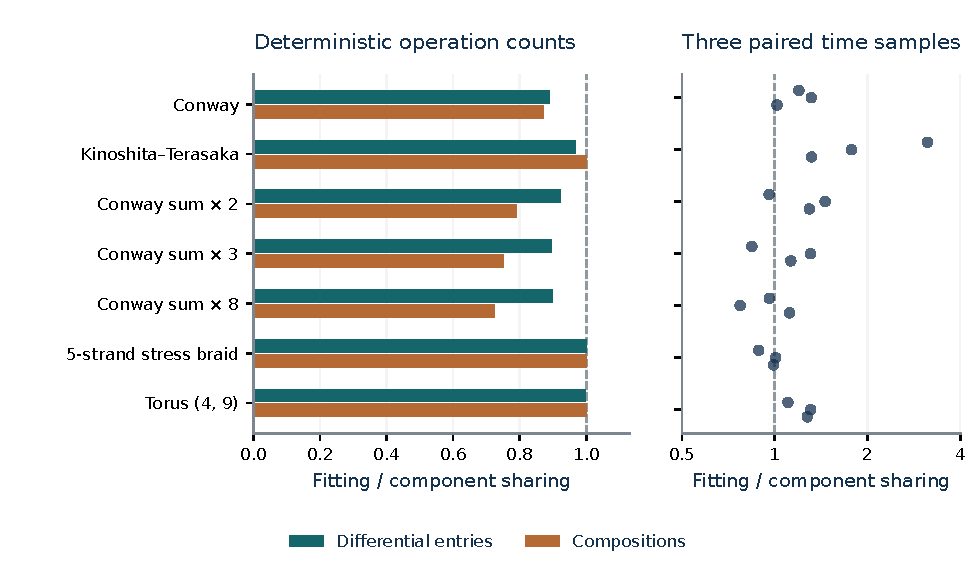
\includegraphics[width=\textwidth]{figures/operations_and_time.pdf}
\caption{Structural work and wall time measure different effects. The left
panel gives exact operation-count ratios for selected cases. Each right-panel
dot is the Fitting/component time ratio in one interleaved repetition on that
case; the time axis is logarithmic. Values below one favor Fitting. The three
dots are measurements, not a confidence interval.}
\label{fig:operations-time}
\end{figure}

\subsection{Wall time, the lazy implementation, and negative results}
The final implementation performs no component copy before an accepted
Fitting split. It does not rebuild the complete arrays if the Fitting or
interval pass makes no change, and it reuses the verified component inventory
across the passes. This matters on diagrams where the search is inactive.
The preceding implementation copied skipped components and exhibited a large
stress-case regression. The archived before/after audit compares 76 completed
result summaries and 380 deterministic statistics with no differences. Both
timing rounds are retained; only the final round supplies the main tables.

In the final round, exact Fitting takes a median 131.92 ms on the eight-fold
Conway sum versus 138.30 ms for component sharing, an observed reduction of
about 4.6\%. The three Fitting samples span 114.07--132.88 ms, while the
component samples span 102.08--170.76 ms. The overlap is substantial. This
small run does not establish a stable speedup. Single Conway and the
three-fold sum are slower with Fitting, at 12.03 versus 10.04 ms and 47.89
versus 42.45 ms, respectively. The stress case is nearly unchanged, 613.22
versus 615.47 ms. The implementation has removed an avoidable overhead, but
has not demonstrated a general wall-clock improvement over the preceding
component backend.

{\small\begin{longtable}{@{}lrrrrrr@{}}
\caption{Median raw scanner time in milliseconds. $S$: standard; $C_s$: preceding component sharing; $F$: exact Fitting; $F_3$: capped decision Fitting. DP preprocessing is included in the last column. $\mathrm{lim}$ denotes three resource-limited calls.}\label{tab:all-timings}\\
\toprule Case & $n$ & $S$ & $C_s$ & $F$ & $F_3$ & $F_3+\mathrm{DP}$\\\midrule
\endfirsthead
\toprule Case & $n$ & $S$ & $C_s$ & $F$ & $F_3$ & $F_3+\mathrm{DP}$\\\midrule
\endhead
\bottomrule\endfoot
$U_8$ & 8 & 2.14 & 1.35 & 2.37 & 1.45 & 2.28\\
$C$ & 11 & 8.94 & 10.04 & 12.03 & 12.53 & 17.18\\
$KT$ & 11 & 10.16 & 8.21 & 12.44 & 14.51 & 17.91\\
$C^{\#2}$ & 22 & 108.70 & 23.50 & 29.36 & 30.83 & 38.19\\
$C^{\#3}$ & 33 & $\mathrm{lim}$ & 42.45 & 47.89 & 46.52 & 61.84\\
$C^{\#8}$ & 88 & $\mathrm{lim}$ & 138.30 & 131.92 & 146.79 & 198.38\\
$B_{5,36}$ & 36 & 520.16 & 615.47 & 613.22 & 635.70 & 867.14\\
$T(3,11)$ & 22 & 12.02 & 12.82 & 12.80 & 9.84 & 17.73\\
$T(4,9)$ & 27 & 50.35 & 54.62 & 71.38 & 63.87 & 70.00\\
$T(5,8)$ & 32 & 545.94 & 618.38 & 607.75 & 629.15 & 619.70\\
$R_{1}$ & 21 & 8.01 & 10.14 & 13.06 & 12.24 & 21.30\\
$R_{2}$ & 23 & 22.25 & 25.00 & 26.48 & 27.92 & 38.11\\
$R_{3}$ & 16 & 2.85 & 3.00 & 4.45 & 3.26 & 8.85\\
$R_{4}$ & 24 & 17.85 & 24.01 & 25.33 & 29.69 & 31.77\\
$R_{5}$ & 23 & 13.78 & 12.54 & 18.14 & 16.07 & 27.06\\
$R_{6}$ & 14 & 2.30 & 2.48 & 2.98 & 4.48 & 6.81\\
$R_{7}$ & 20 & 6.37 & 7.64 & 10.14 & 10.85 & 14.86\\
$R_{8}$ & 24 & 25.25 & 31.51 & 35.98 & 37.36 & 49.77\\
$R_{24}$ & 20 & 9.68 & 12.62 & 16.65 & 16.60 & 31.43\\
\end{longtable}
}

In Table~\ref{tab:all-timings}, $U_8$ denotes the hard unknot, $C$ Conway,
$KT$ Kinoshita--Terasaka, $C^{\#r}$ the supplied $r$-fold connected-sum
diagram, and $B_{5,36}$ the supplied stress braid. The random labels are the
valid-generation indices. Millisecond values below a few milliseconds are
particularly sensitive to interpreter and host variation. The archive
contains every sample, rather than only a best-of-three value.

Decision Fitting also has mixed timings. On this corpus, its difference from
the exact variant concerns multiplicity saturation and degree bookkeeping;
the new interval-length quotient never activates on a nontrivial actual
component. The standard scanner remains the default, while the two new
backends are explicit research options.

\subsection{The interval quotient is currently demonstrated on synthetic complexes}
The most important negative structural observation is exact: across all
nineteen actual diagrams, the interval pass recognizes zero nontrivial whole
common-nilpotent components, including after the accepted scalar splits.
There is consequently no measured knot-diagram speedup attributable to the
new length-two theorem. Actual residual towers carry additional matching
types or differential attachments, so the whole-component hypothesis is
restrictive. Extending the valid continuation quotient to those attached
structures is a principal next research problem.

To verify the implemented transformation itself, the experiment also uses
explicitly constructed legal cobordism complexes. In the first family, eight
layers each contain $q$ copies of one matching, with invertible bidiagonal
scalar matrices multiplied by one dot endomorphism. The differential graph
is connected before the basis change. Exact interval normalization and
sharing turn $8q$ stored objects into eight; decision shortening reduces
those eight to two. At $q=128$, the observed counts are therefore
$1024\to8\to2$.

The second constructed family mixes two matching types and hides $q$ copies
of a three-object complex by a triangular scalar change of basis. For
$q=16$, certified Fitting splitting and exact sharing reduce 48 stored
objects to three. This family tests a transformation that pure-component
recognition cannot perform. Its normalization takes about 83 ms at that
point, illustrating again that a dramatic representation reduction does not
by itself establish an economical search procedure.

\begin{figure}[htbp]
\centering
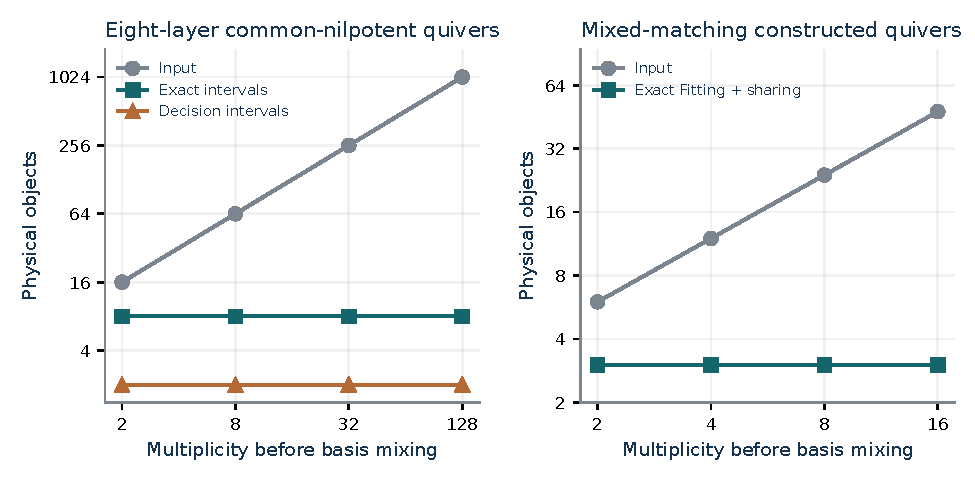
\includegraphics[width=\textwidth]{figures/synthetic_compression.pdf}
\caption{Physical object counts in two constructed algebraic families.
Both axes are logarithmic. These are valid test complexes in the scanner's
category; their realization as intermediate complexes of actual knot
diagrams is not asserted.}
\label{fig:synthetic}
\end{figure}

\subsection{Checkpoint and ordering diagnostics}
The decision scanner records a checkpoint only if every residual component
has actually been classified and normalized as required by the theorem.
The initial state is counted; the final closed state is also a checkpoint.
On single Conway, the maximum observed gap is eleven crossings; the
connected sums retain gap eleven as their number of summands grows. The
stress braid has gap 36, while $T(3,11)$, $T(4,9)$, and $T(5,8)$ have gaps
22, 27, and 32. Their respective maximum frontiers are 8, 6, 8, and 10.
These small measurements support neither a universal logarithmic gap nor
an extrapolation to all hard prime diagrams.

Window optimization improves the declared frontier-mass objective on eight
of the nineteen cases. The peak frontier does not change in these cases.
For example, the Kinoshita--Terasaka mass decreases from 61 to 57, and the
eight-fold Conway sum decreases from 575 to 519. Every accepted order is
verified and all resulting completed ranks agree. However, the preprocessing
cost usually exceeds any downstream saving for a single scan. The stress
case even becomes slower after its mass decreases, showing that the proxy
does not capture the full differential structure.

\begin{table}[htbp]
\centering\small
\begin{tabular}{@{}lrrrr@{}}
\toprule
Case & Initial mass & Final mass & DP time (ms) & Full time (ms)\\\midrule
$KT$ & 61 & 57 & 7.52 & 17.91\\
$C^{\#2}$ & 131 & 123 & 15.29 & 38.19\\
$C^{\#3}$ & 209 & 189 & 24.95 & 61.84\\
$C^{\#8}$ & 575 & 519 & 86.86 & 198.38\\
$B_{5,36}$ & 369 & 353 & 28.22 & 867.14\\
$R_{2}$ & 225 & 221 & 14.44 & 38.11\\
$R_{8}$ & 165 & 161 & 15.36 & 49.77\\
$R_{24}$ & 141 & 125 & 11.32 & 31.43\\
\bottomrule
\end{tabular}

\caption{Every measured case whose frontier-mass objective strictly improves
under window DP. Full time includes DP and the decision scan.}
\label{tab:ordering}
\end{table}

The empirical conclusion is therefore specific. Certified scalar splitting
reduces actual algebraic work on some diagrams. Lazy execution reduces its
avoidable overhead. Exact window optimization improves its own objective.
The interval continuation quotient has a proved asymptotic benefit on its
stated class and is correctly exercised by constructed complexes. A larger
class of active normal forms and a structural checkpoint bound remain
necessary before these ingredients justify a general complexity improvement.

\section{Further research questions and a staged programme}
\label{sec:agenda}

The general target remains open for this implementation. The results above
suggest concrete next questions that can be tested or proved without
assuming the desired state bound. The order below reflects their dependence
on the present code and mathematics.

\subsection{Find the summands before they become large}
The Fitting pass already detects summands that graph connectivity misses.
Its cost currently competes with the time saved by sparser later matrices.
Can the scalar endomorphism space be maintained incrementally when a crossing
is added, instead of solved anew? A useful result would give a complete update
algorithm with cost polynomial in the changed blocks, together with a
criterion deciding when reusing an old splitting remains valid. Every reused
projection must still commute with the new differential.

The current bounded candidate search is deliberately incomplete. A candidate
endomorphism may be invertible or nilpotent on an indecomposable summand and
give no split, even if another endomorphism would work. A next implementation
could use primary decomposition of endomorphisms, or a proved decomposition
algorithm for finite-dimensional module representations. Its cost must be
compared with continuing the unsplit complex. The practical success criterion
is a reduction in complete measured work including decomposition overhead,
not the mere production of additional summands.

\subsection{Extend the class with a finite continuation observation}
The common-$\theta$ condition reduces the problem to the dual numbers. What
is the next useful class? Two independently active dot directions lead toward
\[
 \F[x,y]/(x^2,y^2),
\]
where the classification problem is substantially different. A carefully
scoped goal is to classify continuation observations of a specified family of
two-direction complexes at the rank-two threshold, rather than classify all
modules. The correct statement must quantify over every allowed suffix.
Agreement on sampled closures is evidence for a conjecture, not a valid
replacement rule.

Another useful target is a small tangle with two or more matching types and a
restricted set of saddle maps. The attached towers seen in actual scans
motivate this direction: whole-component common-$\theta$ recognition is too
restrictive on the measured corpus. A normal form for this larger class could
make the present quotient active on ordinary diagrams. Rational-tangle and
four-ended tangle constructions provide relevant prior structure
\cite{thompson,immersed}; their
hypotheses and grading conventions must be retained.

\subsection{Prove a structural bound on the unresolved intervals of a scan}
The checkpoint theorem reduces the target to explicit bounds on $w$ and $g$.
An immediate mathematical question is whether a natural family of validated
diagrams, extending the already tractable braid and rational-tangle families,
admits a constructible order with
\[
 g+2^{w/2}+w\log(w+1)=O((\log n)^2).
\]
A useful theorem must also bound the cost of finding that order. Merely
asserting the existence of a favorable representation would not complete the
algorithmic argument.

Corollary~\ref{cor:coefficient-alphabet} provides another concrete target:
logarithmic frontier width and $O(\log^2 n)$ checkpoint gaps suffice when
the checkpoint coefficients have dot degree at most two. Can a marked,
graded, or restricted-tangle structure force that degree bound after
normalization? The condition concerns actual checkpoint coefficients;
arbitrary intermediate algebra must still be charged in full.

A universal low-width replacement theorem for all knot types is unavailable:
Lunel--de Mesmay give torus-knot families with unavoidable large diagram
treewidth~\cite{widthobstruction}. Such lower bounds do not prevent an
algorithm from rejecting those knots using an inexpensive independent
certificate. This suggests an asymmetric target: either produce a short
nontriviality certificate, or construct a sequence of suitably bounded
algebraic checkpoints. Establishing this dichotomy would be far stronger
than optimizing a handful of observed scans.

\subsection{Build a catalogue of sharp obstructions}
The length-two bound has a sharp formal-block example. Similar sharpness
examples are needed for every proposed observation quotient. In particular,
one should construct common-nilpotent and mixed-matching families whose
serialized component sizes grow, and determine which are realizable inside
actual knot scans. A representation that is legal algebraically need not be
the Khovanov complex of a tangle. Keeping these two questions separate will
prevent synthetic compression demonstrations from being misreported as knot
benchmarks.

The 2026 explicit-basis exponential examples~\cite{kelomaki} are especially
valuable stress families. For each one, record how multiplicity, component
size, scalar endomorphism dimension, and checkpoint gaps grow after each new
normalization. The point is to identify a surviving obstruction, or prove
that an observation quotient removes it, rather than infer asymptotics from
a short timing curve.

\subsection{Exploit graded or marked structure with compatible gluing}
The present exact-rank backend retains homological degree but forgets quantum
degree; decision compression discards still more information. A separate
graded implementation could restrict scalar basis changes to compatible
bigraded blocks and use the grading to constrain possible endomorphisms.
This may lower the cost of the Fitting solver, but could also remove useful
ungraded decompositions. Both outcomes should be measured.

Cohen's characteristic-two splitting of arc algebras is relevant to reducing
the size of the coefficient algebra~\cite{cohen}. The tangle-bimodule result
does not automatically preserve both actions in arbitrary configurations.
A concrete next problem is to specify compatible marked endpoints throughout
the scan and prove that the chosen identifications commute with every gluing
operation. An algebra isomorphism alone does not supply that compatibility.

\subsection{Add a complete tractable topological class}
The linear-time recognition theorem for diagrams of treewidth two provides
an independent complete structural backend~\cite{treewidthtwo}. Implementing
its certified reductions would broaden the front end and offer a useful
comparison with the algebraic route. A proper implementation should accept a
verified decomposition, record every reduction, and distinguish recognition
on the promised class from attempting to discover a suitable diagram.

\subsection{Connect back to compressed hierarchy operations}
The geometric route remains valuable. If an implementation has at most
$L(g+1)^L$ phases and each phase costs at most $B$ bit operations, then
\[
 \log_2 T\le \log_2 B+\log_2 L+L\log_2(g+1)+O(1).
\]
Here the letters are the hierarchy parameters, not the checkpoint gap of
this article. This elementary accounting identity specifies what is needed
from the hierarchy programme: controlled length, controlled pattern data,
and bounded exact operations on the compressed encoding. The July 2026
preprint supplies important pieces~\cite{lackenby2026}; it does not justify
omitting any of these implementation costs.

\subsection{Formalize the new algebraic interface}
The continuation theorem is a manageable formalization target. It can be
split into finite-dimensional linear algebra over $\F$, finite interval
decomposition, the dual-number tensor pairing, and the parity refinement.
The largest foundational dependency is the derived classification; the
appendix provides an explicit elementary route that can be used instead of
importing a general derived-category classification theorem.

A practical first verification milestone is an independently checkable
certificate for each scalar basis split: binary change-of-basis matrices,
their inverses, and the transformed differential. For interval normalization,
rank certificates for the products in the multiplicity formula would certify
the inferred decomposition. Formalizing the observation-preserving shortening
rule then allows a small verifier to accept a decision model without trusting
the optimizer that found it.

\appendix
\section{An elementary dual-number derived classification}
\label{app:dual-number-classification}

This appendix proves the classification used in
Theorem~\ref{thm:rank-formula}, retaining the finiteness conditions needed
for that application. The classification is established mathematics;
see Keller--Yang--Zhou~\cite[Example 3.7(b)]{keller}. The argument here
explains why the possible unbounded projective resolution introduces
only simple-module summands, rather than additional unknown types.

Let $A=\F[\epsilon]/(\epsilon^2)$. A cochain complex has differential
raising its degree by one. A finite free interval $J_l$ has $l$ free
rank-one terms and consecutive differentials $\epsilon$. A
left-infinite interval ending in degree $b$ is
\[
 \cdots\xrightarrow{\epsilon}A
 \xrightarrow{\epsilon}A
 \xrightarrow{\epsilon}\underset{b}{A}\longrightarrow0.
\]
It is exact below $b$ and has cohomology $A/(\epsilon)=\F$ in degree
$b$. It therefore represents a shift of the simple module.

\begin{proposition}[Classification needed for continuation ranks]
\label{prop:derived-classification}
Every bounded complex $D$ of finite-dimensional $A$-modules is
quasi-isomorphic to a finite direct sum of homological shifts of finite
free intervals $J_l$ and of the simple module $\F$.
\end{proposition}

\begin{proof}
We give the construction in three steps.

\paragraph{Step 1: a degreewise finite free resolution.}
There is a bounded-above complex $P$ of finite free $A$-modules and a
quasi-isomorphism $f:P\to D$. The following downward construction
establishes the precise finiteness assertion. Suppose $P$ and $f$ have
been constructed in degrees greater than $i$. The degree-$i$ term of
the partially built mapping cone is $D^i\oplus P^{i+1}$, whose cycles
are the finite $A$-module
\[
 Z_i=\bigl\{(d,p):
 d_Dd+f^{i+1}p=0,\quad d_P^{i+1}p=0\bigr\}.
\]
Choose a finite free module $P^i$ surjecting onto $Z_i$, and define
$f^i$ and $d_P^i$ to be its two component maps. The defining equations
of $Z_i$ give the chain-map identity and $d_P^{i+1}d_P^i=0$.
The new boundaries from $P^i$ in the cone cover all its degree-$i$
cycles. Begin above the highest nonzero degree of $D$ and continue
downward. Each cone degree becomes exact, with its outgoing maps
unaffected by later steps. Hence the completed cone is acyclic.
The resulting $P$ is bounded above and has finite free rank in every
degree, as claimed.

\paragraph{Step 2: minimalization and the exact left tail.}
Over the local ring $A$, cancel every unit entry of the differential,
working downward from the highest degrees. A unit pivot splits off a
contractible pair $A\xrightarrow{\sim}A$. Each pair of adjacent degrees
has finite rank, so only finitely many cancellations are needed there.
Once a differential has all its entries in the radical $(\epsilon)$,
later changes of basis cannot make their residues nonzero. The
descending procedure is locally finite: a fixed degree and its adjacent
matrices stabilize after finitely many operations. It therefore gives
a bounded-above minimal free complex $P'$ quasi-isomorphic to $P$.
This also follows by tracking the elementary cancellation equivalences
degree by degree; no infinite sum of maps in a fixed degree is required.

Write $P'^i=A^{r_i}$. Every differential is now uniquely of the form
\[
 d_{P'}^i=\epsilon B_i,
 \qquad B_i:\F^{r_i}\longrightarrow\F^{r_{i+1}}.
\]
Multiplication by $\epsilon B_i$ has binary rank $\rank(B_i)$:
it maps the constant part to the $\epsilon$ part and kills the latter.
Consequently
\begin{equation}\label{eq:minimal-tail-rank}
 \dim_{\F}H^i(P')
  =2r_i-\rank(B_{i-1})-\rank(B_i).
\end{equation}
Because $D$ is bounded, the left side is zero for every sufficiently
negative $i$. Each rank on the right is at most $r_i$, so exactness in
degree $i$ forces
\[
 \rank(B_{i-1})=\rank(B_i)=r_i.
\]
At two consecutive exact degrees this gives $r_i=r_{i+1}$ and makes
$B_i$ invertible. Hence the sufficiently far-left tail has one constant
finite rank $r$, with every $B_i$ invertible. Choose bases recursively
to make all these tail matrices identities. The case $r=0$ simply
means that the minimal complex is bounded on both sides.

\paragraph{Step 3: one finite interval decomposition.}
Choose a cut degree $a$ within that identity tail. Only finitely many
nonzero degrees lie at or to the right of $a$, and their dimensions
are finite. Apply the elementary finite interval decomposition from
Theorem~\ref{thm:interval} to the sequence of binary matrices from
degree $a$ to the highest degree of $P'$.

Every interval born strictly after $a$ remains a finite interval.
Every interval born at $a$ extends to the left along one of the
identity tail coordinates. To see this explicitly, extend the
chosen change of basis in degree $a$ backward through the identity
tail; all its matrices remain identities. Thus these intervals
become left-infinite intervals, with no additional couplings.
There are finitely many intervals altogether because the finite
sequence being decomposed has finite total dimension.

Reinsert the factor $\epsilon$ in the differentials. This expresses
$P'$ as a finite direct sum of finite free $\epsilon$-intervals and
left-infinite $\epsilon$-intervals. Each left-infinite interval is
quasi-isomorphic to a shifted simple module, as observed above.
Composing with the quasi-isomorphisms in the first two steps proves
the proposition.
\end{proof}

Only existence is needed in the continuation argument. The recognizer
does not construct this resolution for a suffix or attempt to process
an infinite complex. It computes the finite barcode of an already
stored pure component, then applies the rank identity which the
classification proves for every possible suffix.

The distinction between free and arbitrary module continuations matters.
If $D$ is perfect, only finite free intervals occur, so the coefficient
$a$ in~\eqref{eq:continuation-rank-formula} vanishes. In an arbitrary
bounded module complex, shifted simple modules can occur. The geometric
cutoff-two theorem did not assume their absence: it proved that their
number $a$ is even, using the unreduced circle-space parity of the
actual closure. This is why that theorem applies to every square-zero
dot polynomial, including ones whose action is not free on a resolution.

\section{Reproducibility and artifact boundaries}
\label{app:reproduction}

The archive contains the complete \code{fast/} source tree, this article's
\LaTeX\ sources and PDF, deterministic verification programs, paired timing
data, two integration patches, and source provenance. The main package
\code{README.md} gives the shortest entry points; \code{REPRODUCING.md}
describes each experiment and its scope.

The software uses the Python standard library. From \code{fast/}, run
\begin{lstlisting}
python -m unittest discover -s tests -v
python -m fastunknot recognize examples/conway.json --backend fitting
python -m fastunknot khovanov examples/conway.json --fitting
\end{lstlisting}
The last command computes exact ranks with full interval lengths. The
recognition command may return through a preceding structural or polynomial
filter. To reproduce raw backend measurements, use the benchmark script,
whose inputs, backend options, and order selection are recorded in its JSON.

From the package root, the independent continuation check is
\begin{lstlisting}
python verification/verify_continuation.py
\end{lstlisting}
It imports no recognizer module. It enumerates small bounded complexes with
strict square-zero actions, constructs tensor differentials directly as
binary matrices, checks their squares, and compares homology thresholds for
different interval lengths. It also records the counterexamples to an
incorrect universal length-two cutoff without parity and to a geometric
length-one cutoff.

\par\noindent\begin{minipage}{\linewidth}
The article can be rebuilt using
\begin{lstlisting}
sh scripts/build_pdf.sh
\end{lstlisting}
\end{minipage}\par
This requires a standard \LaTeX\ installation with the packages listed in
the preamble. All figure PDFs and generated table fragments needed by the
article are included. Plot regeneration additionally uses Matplotlib; it is
not required to run the recognizer or its mathematical checks.

\subsection{What the records establish}
The source manifest establishes exact byte identity with the stated upstream
files. The patch verification establishes that the supplied textual deltas
reproduce the delivered source from those references. Unit tests establish
the stated finite comparisons; paired timings establish observations on the
recorded host and inputs. None is a substitute for the mathematical
continuation theorem, a proof that every diagram satisfies the checkpoint
condition, or a claim of external peer review.

The included witness data certify individual basis changes, including all
incident maps. An emitted witness is local evidence for a split. The final
recognizer still relies on the established Khovanov unknot-detection theorem
and the implementation of the inherited cobordism algebra.

\subsection{Integration order}
Use the cumulative patch for the pinned repository tree, or the incremental
patch for the already integrated structural 0.3.0 tree. Do not apply both.
The patches target \code{Topology/UnknotRecognition/fast/}. Changes in a
different branch's front-end files should be merged before running the full
combined suite. All reference material redistributed in the package is
project source under the supplied MIT-0 license; third-party papers and
lecture slides are referenced by bibliographic links.

\begin{thebibliography}{99}
\bibitem{proveit}
V. Reshetnikov and contributors,
\emph{ProveIt: Topology/UnknotRecognition}, repository snapshot
\nolinkurl{eb79136d949a1c0e6f4bd2f07e6b3990d1130632}, inspected 7 October 2026.
\url{https://github.com/VladimirReshetnikov/ProveIt/tree/eb79136d949a1c0e6f4bd2f07e6b3990d1130632/Topology/UnknotRecognition}.

\bibitem{prior}
ProveIt research continuation,
\emph{Unknot Recognition by Structural Certificates and Compressed Chain
Complexes}, research article and \code{fastunknot} 0.3.0 package,
7 October 2026, \code{unknot\_structural\_compression.zip}.
Archive identity and reference-code verification are recorded in the
accompanying provenance directory. This is a preceding project artifact,
not an externally reviewed publication.

\bibitem{openaimath}
OpenAI, \emph{math}, repository and formalization scope for family 116,
revision \nolinkurl{adc7f1241b42e322a6451854ab7e4b4c146bf78a}, inspected
7 October 2026.
\url{https://github.com/openai/math/blob/adc7f1241b42e322a6451854ab7e4b4c146bf78a/lean/docs/116.md}.

\bibitem{khovanov}
M. Khovanov, \emph{A functor-valued invariant of tangles},
Algebraic \& Geometric Topology \textbf{2} (2002), 665--741.
\url{https://arxiv.org/abs/math/0103190}.

\bibitem{barnatan}
D. Bar-Natan, \emph{Khovanov's homology for tangles and cobordisms},
Geometry \& Topology \textbf{9} (2005), 1443--1499.
\url{https://arxiv.org/abs/math/0410495}.

\bibitem{bnfast}
D. Bar-Natan, \emph{Fast Khovanov homology computations},
Journal of Knot Theory and Its Ramifications \textbf{16} (2007), 243--255.
\url{https://arxiv.org/abs/math/0606318}.

\bibitem{carlsson}
G. Carlsson and V. de Silva, \emph{Zigzag persistence},
Foundations of Computational Mathematics \textbf{10} (2010), 367--405.
The interval classification is attributed there to Gabriel; see Theorem 2.5
and the constructive treatment in Section 4.
\url{https://arxiv.org/abs/0812.0197}.

\bibitem{keller}
B. Keller, D. Yang, and G. Zhou,
\emph{The Hall algebra of a spherical object},
Journal of the London Mathematical Society \textbf{80} (2009), 771--784;
arXiv:0810.5546v2 (2008).
Example 3.7(b) records the required classification over $R/(\pi^2)$.
\url{https://arxiv.org/abs/0810.5546}.

\bibitem{km}
P. B. Kronheimer and T. S. Mrowka,
\emph{Khovanov homology is an unknot-detector},
Publications Math\'ematiques de l'IH\'ES \textbf{113} (2011), 97--208.
\url{https://arxiv.org/abs/1005.4346}.

\bibitem{shumakovitch}
A. Shumakovitch, \emph{Torsion of Khovanov homology},
Fundamenta Mathematicae \textbf{225} (2014), 343--364.
Corollary 3.2.C gives the characteristic-two splitting.
\url{https://arxiv.org/abs/math/0405474}.

\bibitem{kelomaki}
T. Kelom\"aki and D. Sch\"utz,
\emph{On computational complexity of Khovanov homology},
arXiv:2601.02119v1 (5 January 2026).
\url{https://arxiv.org/abs/2601.02119}.

\bibitem{lackenbytalk}
M. Lackenby, \emph{The unknot recognition problem},
Oxford lecture slides (2021), including the announced quasi-polynomial bound.
\url{https://people.maths.ox.ac.uk/lackenby/quasipolynomial-talk-oxford.pdf}.
The slides are cited but not redistributed.

\bibitem{lackenby2026}
M. Lackenby, \emph{Incompressible surfaces, hierarchies and unknot recognition},
arXiv:2607.23350v1 (25 July 2026), especially Section 9 and Proposition 9.1.
\url{https://arxiv.org/abs/2607.23350}.

\bibitem{treewidthtwo}
H. L. Bodlaender, B. A. Burton, F. V. Fomin, and A. Grigoriev,
\emph{Knot diagrams of treewidth two}, WG 2020;
arXiv:1904.03117.
\url{https://arxiv.org/abs/1904.03117}.

\bibitem{widthobstruction}
C. Lunel and A. de Mesmay,
\emph{A structural approach to tree decompositions of knots and spatial graphs},
Algebraic \& Geometric Topology \textbf{26} (2026), 2015--2047;
arXiv:2303.07982v2.
\url{https://arxiv.org/abs/2303.07982}.

\bibitem{cohen}
J. Cohen, \emph{An exceptional splitting of Khovanov's arc algebras in
characteristic 2}, Fundamenta Mathematicae \textbf{264} (2024), 69--84;
arXiv:2209.01705. The algebra splitting and limitations of bimodule
compatibility appear in Theorem 3.2 and
Proposition 3.3 of that manuscript.
\url{https://arxiv.org/abs/2209.01705}.

\bibitem{thompson}
B. Thompson, \emph{Khovanov complexes of rational tangles},
arXiv:1701.07525v2 (2018).
\url{https://arxiv.org/abs/1701.07525}.

\bibitem{immersed}
A. Kotelskiy, L. Watson, and C. Zibrowius,
\emph{Immersed curves in Khovanov homology},
arXiv:1910.14584.
\url{https://arxiv.org/abs/1910.14584}.
\end{thebibliography}

\end{document}
